
%% bare_conf.tex
%% V1.4b
%% 2015/08/26
%% by Michael Shell
%% See:
%% http://www.michaelshell.org/
%% for current contact information.
%%
%% This is a skeleton file demonstrating the use of IEEEtran.cls
%% (requires IEEEtran.cls version 1.8b or later) with an IEEE
%% conference paper.
%%
%% Support sites:
%% http://www.michaelshell.org/tex/ieeetran/
%% http://www.ctan.org/pkg/ieeetran
%% and
%% http://www.ieee.org/

%%*************************************************************************
%% Legal Notice:
%% This code is offered as-is without any warranty either expressed or
%% implied; without even the implied warranty of MERCHANTABILITY or
%% FITNESS FOR A PARTICULAR PURPOSE! 
%% User assumes all risk.
%% In no event shall the IEEE or any contributor to this code be liable for
%% any damages or losses, including, but not limited to, incidental,
%% consequential, or any other damages, resulting from the use or misuse
%% of any information contained here.
%%
%% All comments are the opinions of their respective authors and are not
%% necessarily endorsed by the IEEE.
%%
%% This work is distributed under the LaTeX Project Public License (LPPL)
%% ( http://www.latex-project.org/ ) version 1.3, and may be freely used,
%% distributed and modified. A copy of the LPPL, version 1.3, is included
%% in the base LaTeX documentation of all distributions of LaTeX released
%% 2003/12/01 or later.
%% Retain all contribution notices and credits.
%% ** Modified files should be clearly indicated as such, including  **
%% ** renaming them and changing author support contact information. **
%%*************************************************************************


% *** Authors should verify (and, if needed, correct) their LaTeX system  ***
% *** with the testflow diagnostic prior to trusting their LaTeX platform ***
% *** with production work. The IEEE's font choices and paper sizes can   ***
% *** trigger bugs that do not appear when using other class files.       ***                          ***
% The testflow support page is at:
% http://www.michaelshell.org/tex/testflow/



\documentclass[conference]{IEEEtran}
% Some Computer Society conferences also require the compsoc mode option,
% but others use the standard conference format.
%
% If IEEEtran.cls has not been installed into the LaTeX system files,
% manually specify the path to it like:
% \documentclass[conference]{../sty/IEEEtran}





% Some very useful LaTeX packages include:
% (uncomment the ones you want to load)


% *** MISC UTILITY PACKAGES ***
%
%\usepackage{ifpdf}
% Heiko Oberdiek's ifpdf.sty is very useful if you need conditional
% compilation based on whether the output is pdf or dvi.
% usage:
% \ifpdf
%   % pdf code
% \else
%   % dvi code
% \fi
% The latest version of ifpdf.sty can be obtained from:
% http://www.ctan.org/pkg/ifpdf
% Also, note that IEEEtran.cls V1.7 and later provides a builtin
% \ifCLASSINFOpdf conditional that works the same way.
% When switching from latex to pdflatex and vice-versa, the compiler may
% have to be run twice to clear warning/error messages.






% *** CITATION PACKAGES ***
%
%\usepackage{cite}
% cite.sty was written by Donald Arseneau
% V1.6 and later of IEEEtran pre-defines the format of the cite.sty package
% \cite{} output to follow that of the IEEE. Loading the cite package will
% result in citation numbers being automatically sorted and properly
% "compressed/ranged". e.g., [1], [9], [2], [7], [5], [6] without using
% cite.sty will become [1], [2], [5]--[7], [9] using cite.sty. cite.sty's
% \cite will automatically add leading space, if needed. Use cite.sty's
% noadjust option (cite.sty V3.8 and later) if you want to turn this off
% such as if a citation ever needs to be enclosed in parenthesis.
% cite.sty is already installed on most LaTeX systems. Be sure and use
% version 5.0 (2009-03-20) and later if using hyperref.sty.
% The latest version can be obtained at:
% http://www.ctan.org/pkg/cite
% The documentation is contained in the cite.sty file itself.






% *** GRAPHICS RELATED PACKAGES ***
%
\ifCLASSINFOpdf
   \usepackage[pdftex]{graphicx}
  % declare the path(s) where your graphic files are
   \graphicspath{{./Abbildungen/}}
  % and their extensions so you won't have to specify these with
  % every instance of \includegraphics
   \DeclareGraphicsExtensions{.pdf}
\else
  % or other class option (dvipsone, dvipdf, if not using dvips). graphicx
  % will default to the driver specified in the system graphics.cfg if no
  % driver is specified.
  % \usepackage[dvips]{graphicx}
  % declare the path(s) where your graphic files are
  % \graphicspath{{../eps/}}
  % and their extensions so you won't have to specify these with
  % every instance of \includegraphics
  % \DeclareGraphicsExtensions{.eps}
\fi
% graphicx was written by David Carlisle and Sebastian Rahtz. It is
% required if you want graphics, photos, etc. graphicx.sty is already
% installed on most LaTeX systems. The latest version and documentation
% can be obtained at: 
% http://www.ctan.org/pkg/graphicx
% Another good source of documentation is "Using Imported Graphics in
% LaTeX2e" by Keith Reckdahl which can be found at:
% http://www.ctan.org/pkg/epslatex
%
% latex, and pdflatex in dvi mode, support graphics in encapsulated
% postscript (.eps) format. pdflatex in pdf mode supports graphics
% in .pdf, .jpeg, .png and .mps (metapost) formats. Users should ensure
% that all non-photo figures use a vector format (.eps, .pdf, .mps) and
% not a bitmapped formats (.jpeg, .png). The IEEE frowns on bitmapped formats
% which can result in "jaggedy"/blurry rendering of lines and letters as
% well as large increases in file sizes.
%
% You can find documentation about the pdfTeX application at:
% http://www.tug.org/applications/pdftex





% *** MATH PACKAGES ***
%
\usepackage{amsmath}
% A popular package from the American Mathematical Society that provides
% many useful and powerful commands for dealing with mathematics.
%
% Note that the amsmath package sets \interdisplaylinepenalty to 10000
% thus preventing page breaks from occurring within multiline equations. Use:
%\interdisplaylinepenalty=2500
% after loading amsmath to restore such page breaks as IEEEtran.cls normally
% does. amsmath.sty is already installed on most LaTeX systems. The latest
% version and documentation can be obtained at:
% http://www.ctan.org/pkg/amsmath

\usepackage{amssymb}



% *** SPECIALIZED LIST PACKAGES ***
%
%\usepackage{algorithmic}
% algorithmic.sty was written by Peter Williams and Rogerio Brito.
% This package provides an algorithmic environment fo describing algorithms.
% You can use the algorithmic environment in-text or within a figure
% environment to provide for a floating algorithm. Do NOT use the algorithm
% floating environment provided by algorithm.sty (by the same authors) or
% algorithm2e.sty (by Christophe Fiorio) as the IEEE does not use dedicated
% algorithm float types and packages that provide these will not provide
% correct IEEE style captions. The latest version and documentation of
% algorithmic.sty can be obtained at:
% http://www.ctan.org/pkg/algorithms
% Also of interest may be the (relatively newer and more customizable)
% algorithmicx.sty package by Szasz Janos:
% http://www.ctan.org/pkg/algorithmicx




% *** ALIGNMENT PACKAGES ***
%
%\usepackage{array}
% Frank Mittelbach's and David Carlisle's array.sty patches and improves
% the standard LaTeX2e array and tabular environments to provide better
% appearance and additional user controls. As the default LaTeX2e table
% generation code is lacking to the point of almost being broken with
% respect to the quality of the end results, all users are strongly
% advised to use an enhanced (at the very least that provided by array.sty)
% set of table tools. array.sty is already installed on most systems. The
% latest version and documentation can be obtained at:
% http://www.ctan.org/pkg/array


% IEEEtran contains the IEEEeqnarray family of commands that can be used to
% generate multiline equations as well as matrices, tables, etc., of high
% quality.




% *** SUBFIGURE PACKAGES ***
%\ifCLASSOPTIONcompsoc
%  \usepackage[caption=false,font=normalsize,labelfont=sf,textfont=sf]{subfig}
%\else
%  \usepackage[caption=false,font=footnotesize]{subfig}
%\fi
% subfig.sty, written by Steven Douglas Cochran, is the modern replacement
% for subfigure.sty, the latter of which is no longer maintained and is
% incompatible with some LaTeX packages including fixltx2e. However,
% subfig.sty requires and automatically loads Axel Sommerfeldt's caption.sty
% which will override IEEEtran.cls' handling of captions and this will result
% in non-IEEE style figure/table captions. To prevent this problem, be sure
% and invoke subfig.sty's "caption=false" package option (available since
% subfig.sty version 1.3, 2005/06/28) as this is will preserve IEEEtran.cls
% handling of captions.
% Note that the Computer Society format requires a larger sans serif font
% than the serif footnote size font used in traditional IEEE formatting
% and thus the need to invoke different subfig.sty package options depending
% on whether compsoc mode has been enabled.
%
% The latest version and documentation of subfig.sty can be obtained at:
% http://www.ctan.org/pkg/subfig




% *** FLOAT PACKAGES ***
%
%\usepackage{fixltx2e}
% fixltx2e, the successor to the earlier fix2col.sty, was written by
% Frank Mittelbach and David Carlisle. This package corrects a few problems
% in the LaTeX2e kernel, the most notable of which is that in current
% LaTeX2e releases, the ordering of single and double column floats is not
% guaranteed to be preserved. Thus, an unpatched LaTeX2e can allow a
% single column figure to be placed prior to an earlier double column
% figure.
% Be aware that LaTeX2e kernels dated 2015 and later have fixltx2e.sty's
% corrections already built into the system in which case a warning will
% be issued if an attempt is made to load fixltx2e.sty as it is no longer
% needed.
% The latest version and documentation can be found at:
% http://www.ctan.org/pkg/fixltx2e


%\usepackage{stfloats}
% stfloats.sty was written by Sigitas Tolusis. This package gives LaTeX2e
% the ability to do double column floats at the bottom of the page as well
% as the top. (e.g., "\begin{figure*}[!b]" is not normally possible in
% LaTeX2e). It also provides a command:
%\fnbelowfloat
% to enable the placement of footnotes below bottom floats (the standard
% LaTeX2e kernel puts them above bottom floats). This is an invasive package
% which rewrites many portions of the LaTeX2e float routines. It may not work
% with other packages that modify the LaTeX2e float routines. The latest
% version and documentation can be obtained at:
% http://www.ctan.org/pkg/stfloats
% Do not use the stfloats baselinefloat ability as the IEEE does not allow
% \baselineskip to stretch. Authors submitting work to the IEEE should note
% that the IEEE rarely uses double column equations and that authors should try
% to avoid such use. Do not be tempted to use the cuted.sty or midfloat.sty
% packages (also by Sigitas Tolusis) as the IEEE does not format its papers in
% such ways.
% Do not attempt to use stfloats with fixltx2e as they are incompatible.
% Instead, use Morten Hogholm'a dblfloatfix which combines the features
% of both fixltx2e and stfloats:
%
% \usepackage{dblfloatfix}
% The latest version can be found at:
% http://www.ctan.org/pkg/dblfloatfix




% *** PDF, URL AND HYPERLINK PACKAGES ***
%
%\usepackage{url}
% url.sty was written by Donald Arseneau. It provides better support for
% handling and breaking URLs. url.sty is already installed on most LaTeX
% systems. The latest version and documentation can be obtained at:
% http://www.ctan.org/pkg/url
% Basically, \url{my_url_here}.




% *** Do not adjust lengths that control margins, column widths, etc. ***
% *** Do not use packages that alter fonts (such as pslatex).         ***
% There should be no need to do such things with IEEEtran.cls V1.6 and later.
% (Unless specifically asked to do so by the journal or conference you plan
% to submit to, of course. )


% correct bad hyphenation here
\hyphenation{op-tical net-works semi-conduc-tor}

%------------------------Thilo Package Area-----------------------------
%Package for writing german letters
\usepackage[utf8]{inputenc}

%-----------------------------------------------------------------------
\begin{document}
%
% paper title
% Titles are generally capitalized except for words such as a, an, and, as,
% at, but, by, for, in, nor, of, on, or, the, to and up, which are usually
% not capitalized unless they are the first or last word of the title.
% Linebreaks \\ can be used within to get better formatting as desired.
% Do not put math or special symbols in the title.
\title{(Deep) Reinforcement Learning - \\ Policy Gradient}


% author names and affiliations
% use a multiple column layout for up to three different
% affiliations
\author{\IEEEauthorblockN{Thilo Stegemann}
\IEEEauthorblockA{Hochschule für Technik und Wirtschaft\\Master Student der Angewandten Informatik\\
12459 Berlin, Wilhelminenhofstraße 75A\\
Email: t.stegemann@gmx.de}}

% conference papers do not typically use \thanks and this command
% is locked out in conference mode. If really needed, such as for
% the acknowledgment of grants, issue a \IEEEoverridecommandlockouts
% after \documentclass

% for over three affiliations, or if they all won't fit within the width
% of the page, use this alternative format:
% 
%\author{\IEEEauthorblockN{Michael Shell\IEEEauthorrefmark{1},
%Homer Simpson\IEEEauthorrefmark{2},
%James Kirk\IEEEauthorrefmark{3}, 
%Montgomery Scott\IEEEauthorrefmark{3} and
%Eldon Tyrell\IEEEauthorrefmark{4}}
%\IEEEauthorblockA{\IEEEauthorrefmark{1}School of Electrical and Computer Engineering\\
%Georgia Institute of Technology,
%Atlanta, Georgia 30332--0250\\ Email: see http://www.michaelshell.org/contact.html}
%\IEEEauthorblockA{\IEEEauthorrefmark{2}Twentieth Century Fox, Springfield, USA\\
%Email: homer@thesimpsons.com}
%\IEEEauthorblockA{\IEEEauthorrefmark{3}Starfleet Academy, San Francisco, California 96678-2391\\
%Telephone: (800) 555--1212, Fax: (888) 555--1212}
%\IEEEauthorblockA{\IEEEauthorrefmark{4}Tyrell Inc., 123 Replicant Street, Los Angeles, California 90210--4321}}




% use for special paper notices
%\IEEEspecialpapernotice{(Invited Paper)}




% make the title area
\maketitle

% As a general rule, do not put math, special symbols or citations
% in the abstract
\begin{abstract}
Die Policy Gradient Verfahren sind Methoden zum lernen optimaler stochastischer Strategiefunktion (Policy) in unbekannten Markov-Entscheidungsprozessen. Die zu lernende Strategiefunktion wird parametrisiert und mittels einer linearen Kombination von Merkmalen oder einem Neuronalen Netz an eine unbekannte wahre optimale Strategie angenähert. Die Policy Gradient Verfahren aktualisieren die Parameter der Strategiefunktion in Richtung des Gradienten einer Zielfunktion. Ziel dieser Arbeit ist, dass allgemeine Verständnis des Policy Gradient Verfahrens für Probleme des Reinforcement Learnings. Policy Gradient Verfahren sollen es ermöglichen diverse Computerspiele, Robotersteuerungen, Fahrzeugsteuerungen und anderes zu lernen.
\end{abstract}

% no keywords




% For peer review papers, you can put extra information on the cover
% page as needed:
% \ifCLASSOPTIONpeerreview
% \begin{center} \bfseries EDICS Category: 3-BBND \end{center}
% \fi
%
% For peerreview papers, this IEEEtran command inserts a page break and
% creates the second title. It will be ignored for other modes.
\IEEEpeerreviewmaketitle

% An example of a floating figure using the graphicx package.
% Note that \label must occur AFTER (or within) \caption.
% For figures, \caption should occur after the \includegraphics.
% Note that IEEEtran v1.7 and later has special internal code that
% is designed to preserve the operation of \label within \caption
% even when the captionsoff option is in effect. However, because
% of issues like this, it may be the safest practice to put all your
% \label just after \caption rather than within \caption{}.
%
% Reminder: the "draftcls" or "draftclsnofoot", not "draft", class
% option should be used if it is desired that the figures are to be
% displayed while in draft mode.
%
%\begin{figure}[!t]
%\centering
%\includegraphics[width=2.5in]{myfigure}
% where an .eps filename suffix will be assumed under latex, 
% and a .pdf suffix will be assumed for pdflatex; or what has been declared
% via \DeclareGraphicsExtensions.
%\caption{Simulation results for the network.}
%\label{fig_sim}
%\end{figure}

% Note that the IEEE typically puts floats only at the top, even when this
% results in a large percentage of a column being occupied by floats.


% An example of a double column floating figure using two subfigures.
% (The subfig.sty package must be loaded for this to work.)
% The subfigure \label commands are set within each subfloat command,
% and the \label for the overall figure must come after \caption.
% \hfil is used as a separator to get equal spacing.
% Watch out that the combined width of all the subfigures on a 
% line do not exceed the text width or a line break will occur.
%
%\begin{figure*}[!t]
%\centering
%\subfloat[Case I]{\includegraphics[width=2.5in]{box}%
%\label{fig_first_case}}
%\hfil
%\subfloat[Case II]{\includegraphics[width=2.5in]{box}%
%\label{fig_second_case}}
%\caption{Simulation results for the network.}
%\label{fig_sim}
%\end{figure*}
%
% Note that often IEEE papers with subfigures do not employ subfigure
% captions (using the optional argument to \subfloat[]), but instead will
% reference/describe all of them (a), (b), etc., within the main caption.
% Be aware that for subfig.sty to generate the (a), (b), etc., subfigure
% labels, the optional argument to \subfloat must be present. If a
% subcaption is not desired, just leave its contents blank,
% e.g., \subfloat[].


% An example of a floating table. Note that, for IEEE style tables, the
% \caption command should come BEFORE the table and, given that table
% captions serve much like titles, are usually capitalized except for words
% such as a, an, and, as, at, but, by, for, in, nor, of, on, or, the, to
% and up, which are usually not capitalized unless they are the first or
% last word of the caption. Table text will default to \footnotesize as
% the IEEE normally uses this smaller font for tables.
% The \label must come after \caption as always.
%
%\begin{table}[!t]
%% increase table row spacing, adjust to taste
%\renewcommand{\arraystretch}{1.3}
% if using array.sty, it might be a good idea to tweak the value of
% \extrarowheight as needed to properly center the text within the cells
%\caption{An Example of a Table}
%\label{table_example}
%\centering
%% Some packages, such as MDW tools, offer better commands for making tables
%% than the plain LaTeX2e tabular which is used here.
%\begin{tabular}{|c||c|}
%\hline
%One & Two\\
%\hline
%Three & Four\\
%\hline
%\end{tabular}
%\end{table}


% Note that the IEEE does not put floats in the very first column
% - or typically anywhere on the first page for that matter. Also,
% in-text middle ("here") positioning is typically not used, but it
% is allowed and encouraged for Computer Society conferences (but
% not Computer Society journals). Most IEEE journals/conferences use
% top floats exclusively. 
% Note that, LaTeX2e, unlike IEEE journals/conferences, places
% footnotes above bottom floats. This can be corrected via the
% \fnbelowfloat command of the stfloats package.

% conference papers do not normally have an appendix


\section{Reinforcement Learning (RL)}
Sutton und Barto \cite{sutton_barto_12} definieren ein Standard Reinforcement Learning Framework, in diesem interagiert ein Agent mit einer Umgebung. Dieses standart RL-Framework wird nachfolgend ausführlich beschrieben, denn es ist eine elementare Grundlage für das Verständnis des Policy Gradient Verfahrens. Die Wertefunktionsapproximation und die Strategiefunktionsapproximation basieren auf den Ausführungen von D. Silver vgl. \cite{silver_15}, diese Funktionen sind ebenfalls Grundlegend für das Verständnis des Policy Gradient Verfahrens.

\subsection{Markov-Entscheidungsprozess}
Der Agent lernt, in einer ihm unbekannten Umgebung, durch Versuch und Irrtum eine Strategie $\pi$ (eng. Policy). Der Agent kann in einer bestimmten Umgebung bestimmte Aktionen $a$ ausführen. Ist die Menge der Aktionen begrenzt, dann ist es ein diskreter Aktionsraum $A$. Eine unbegrenzte Menge von Aktionen bezeichnet einen kontinuierlichen Aktionsraum. Die Umgebung bestimmt die Aktionsmenge und der Agent entscheidet welche Aktion aus dieser Menge ausgewählt wird. Eine Aktion kann eine Positionsangabe, eine Richtung oder etwas viel komplexeres sein. Die Umgebung ist ein Markov-Entscheidungsprozess (eng. \textbf{M}arkov \textbf{D}ecision \textbf{P}rocess, kurz MDP). Der Agent interagiert demnach mit einem MDP und erhält von diesem einen Zustand und eine Belohnung. Das MDP erhält vom Agenten eine ausgewählte Aktion. Ein MDP ist ein sequentielles Entscheidungsproblem. Eine Sequenz $... S_t, A_t, R_{t+1}, S_{t+1}, A_{t+1}, R_{t+2}, S_{t+2} ...$ beschreibt die Interaktion des Agenten mit dem MDP. Ein Zustand ist eine Darstellung der Umwelt zu einem Zeitpunkt t. Die Zustände bestimmten, welche Aktionen ausgeführt werden können d.h. es existiert eine Funktion $A(S_t)$. Ergebnis dieser Funktion ist eine zulässige Menge von Aktionen $A_t$ in einem Zustand $S_t$. Der Agent erhält eine direkte Belohnung $R_{t+1}$ für das Ausführen einer Aktion $A_t$ in einem Zustand $S_t$.
\paragraph*{Ein Beispiel} ein Modellhubschrauber soll eigenständig lernen zu fliegen ohne abzustürzen und bestimmte Manöver auszuführen. In diesem Beispiel ist die Steuerung des Modellhubschraubers die zu lernende Strategie des RL Algorithmus. Eigenschaften der Umwelt sind unter anderem: Luftdruck, Position und Geschwindigkeit des Hubschraubers, Windgeschwindigkeit, Treibstoff. All diese Eigenschaften kombiniert bilden einen Zustand $S_t$ zu einem Zeitpunkt $t$ ab. Zustände und Aktionen können sehr komplexe Objekte sein, dahingegen ist die Belohnung ein numerischer Wert und kein komplexes Objekt.

Die numerische Belohnung ist eine Bewertung der Aktion des Agenten. Der Agent versucht diese numerische Belohnung, über die Zeit, zu maximieren. Der Agent kann eine Belohnung von $+10$ erhalten (Hubschrauber um 360 Grad gedreht), wenn er in einem Zustand $s$ eine Aktion $a$ mit $s\in S$ und $a\in A$ ausführt. Der Agent kann auch eine negative numerische Belohnung von z.B. $-23$ erhalten (Hubschrauber abgestürzt). Der genaue Wert der Belohnung wird von der Umgebung definiert und der Agent kann diesen Wert nicht direkt beeinflussen oder verändern. Allein die Entscheidungen d.h. die Aktionsauswahl des Agenten entscheidet über die erhaltene direkte Belohnung $r$. Die Umgebung definiert eine Belohnungsfunktion $R_s^a = \mathbb{E}\{ r_{t+1} | s_t = s, a_t = a \}$. Diese Funktion ist eine Abbildung von Zustand-Aktionspaaren auf erwartete Belohnungen.

In einer realen Umgebung kann es passieren, dass der Agent selbst (z.B. ein einfacher Laufroboter oder ein Hubschrauber) eine Signalstörung empfängt oder eine Fehlfunktion seiner mechanischen Steuereinheiten hat. Die Umgebungsgegebenheiten können sich ebenfalls verschieben oder verändern (z.B. wechselnde Windrichtungen, Windstärken-Schwankungen, andere autonom agierende Agenten). Man bezeichnet diese Möglichkeiten als die Dynamiken der Umgebung. Abgebildet werden diese Dynamiken mittels Wahrscheinlichkeiten. Die Zustandsübergangswahrscheinlichkeit das ein Agent in Zustand $s_t$ mit der Aktion $a_t$ in den Zustand $s'_t$ übergeht ist definiert durch die Wahrscheinlichkeit $P^a_{ss'} = Pr \{ s_{t+1} = s' | s_t = s, a_t = a \}$ (auch als Umgebungsdynamik bezeichnet).

\subsection{Wertefunktionsapproximation}
Eine nicht approximierte Wertefunktion ist eine Wertetabelle. In dieser Wertetabelle hat jeder Zustand $s$ einen Eintrag der Form $V(s)$ oder jedes Zustands-Aktionspaar $s, a$ hat einen Eintrag $Q(s,a)$. Für große Markov-Entscheidungsprozesse existieren zu viele Zustände und Aktionen, um diese in der Wertetabelle speichern zu können. Das eigentliche Lernen der Wertefunktion ist zudem sehr langsam, weil für jeden Zustand ein individueller Wert gelernt werden muss. Die Lösung für große MDPs ist daher eine geschätzte (eng. estimated) Wertefunktion. Die Schätzung erfolgt mittels Funktionsapproximation:

$V_{\theta}(s) \approx V^{\pi}(s)$, dabei ist $V^{\pi}(s)$ die wahre Zustands-Wertefunktion, diese definiert wie viel erwartete Belohnung kann der Agent wirklich erhalten, wenn er der Strategie $\pi$ folgt und sich in Zustand $s$ befindet.

$Q_{\theta}(s, a) \approx Q^{\pi}(s, a)$, dabei ist $Q^{\pi}(s, a)$ die wahre Q-Funktion, welche für ein Zustands-Aktionspaar $s, a$ definiert, wie hoch die wahre zu erwartende akkumulierte Belohnung ist, unter Berücksichtigung der Strategie $\pi$.

$V_{\theta}(s)$ und $Q_{\theta}(s, a)$ sind Funktionsapproximationen, welche sich an die wahren Wertefunktionen annähern sollen. Die approximierten Funktionen generalisieren von bereits besuchten/bekannten Zuständen auf unbekannte/noch nicht besuchte Zustände. In der Regeln ist die Anzahl der Parameter im Parametervektor $\theta$ viel kleiner als die Anzahl der Zustände des MDPs. Die Annäherung erfolgt durch die Modifikation des Parametervektors $\theta$ (wird auch oft als $w$ bezeichnet). Dieser Parametervektor wird mittels Monte-Carlo oder Temporaler-Differenz gelernt. Im nächsten Abschnitt wird das gerade beschriebene Konzept der Funktionsapproximation auf die Strategiefunktion angewendet.
%
%\begin{figure}[!t]
%\centering
%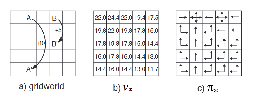
\includegraphics[width=3.5in]{gridworld_example}
%\caption{Optimale Lösungen des Rasterwelt Beispiels nach \cite{sutton_barto_12}.}
%\label{gridworld_example}
%\end{figure}

\subsection{Strategiefunktionsapproximation}
Eine Strategie $\pi$ (eng. Policy) definiert das Verhalten des Agenten als Funktion von Zuständen $s$, mit $s \in S$ und $S$ ist der gesamte Zustandsraum des MDPs. Bei allen Wertefunktionsbasierten Methoden wird eine Wertefunktion gelernt und mittels dieser kann implizit eine Strategie erstellt werden (z.B. mit $\epsilon-greedy$ vgl. \cite{silver_15}). Innerhalb dieser Arbeit werden speziell die Methoden erläutert, welche Strategien $\pi_\theta$ (bzw. den Parametervektor $\theta$) direkt lernen. Eine stochastische approximierte Strategiefunktion wird als $\pi(s,a,\theta) = Pr \{ a_t = a | s_t = s, \theta \}$ geschrieben. $\pi(s,a,\theta)$ wird oft auch als $\pi(s,a)$ geschrieben. Die Strategie ist stochastisch (nicht-deterministisch) d.h. sie beschreibt Wahrscheinlichkeiten für das Auswählen von Aktionen. Eine deterministische (nicht-stochastische) Strategie legt jeweils exakt eine Aktion für einen Zustand fest. Eine weitere Beschreibung der Strategiefunktion wäre $\pi_\theta (s,a) = P[a|s,\theta]$, d.h. $\pi_\theta (s,a)$ gibt die Wahrscheinlichkeitsverteilung über den möglichen Aktionen $a$ im Zustand $s$ an und durch den Parametervektor $\theta$ kann diese Wahrscheinlichkeitsverteilung verändert werden. Das optimieren des Parametervektors $\theta$ der Strategiefunktion $\pi_\theta$ ist Ziel des Policy Gradient Verfahrens und wird im nächsten Abschnitt ausführlich behandelt. 

\section{Policy Gradient}
Die nachfolgenden Erläuterungen basieren auf der wissenschaftlichen Arbeit unter anderem von R. S. Sutton \cite{sutton_99}, D. Silver \cite{silver_15} und G. Hoever \cite[vgl. S. 213 f]{hoever_14}. Der Agent soll eine approximierte stochastische optimale Strategie $\pi_\theta (s, a)$ mittels des Policy Gradienten Verfahrens erlernen. Für ein besseres Verständnis des Policy Gradient Verfahrens wird zuerst die allgemeine gradientenbasierte lokale Optimierung erläutert und anschließend wird erklärt was eine Zielfunktion ist und wie diese dargestellt werden kann. Die letzten beiden Teilabschnitte beschreiben die Anwendung des Gradientenverfahrens auf die Zielfunktion und eine Unterscheidung verschiedener Policy Gradient Methoden.

\subsection{Gradientenbasierte lokale Optimierung}
In einem Gradienten werden die verschiedenen partiellen Ableitungen einer Zielfunktion $J(\theta)$ zusammengefasst. Zu einer Zielfunktion $J : \mathbb{R}^n \rightarrow \mathbb{R}$ heißt (falls die partiellen Ableitungen existieren)

\begin{equation*}
\nabla_\theta J(\theta) := grad \: J(\theta) := \begin{pmatrix}
\frac{\partial J(\theta)}{\partial \theta_1}, \hdots, \frac{\partial J(\theta)}{\partial \theta_n}
\end{pmatrix}
\end{equation*}

Gradient von $J$ im Punkt $\theta$. ($\nabla J$ wird "nabla $J$" gelesen.) Der Gradient einer Funktion weist in die Richtung des Steilsten Anstiegs. Senkrecht zum Gradienten ändert sich der Funktionswert nicht. Sucht man ausgehend von einem Startpunkt $\theta^{(0)}$ eine Maximalstelle (Gradient Ascent), so geht man ein Stück in die Richtung des Gradienten, also
\begin{equation*}
\theta^{(1)} = \theta^{(0)} + \alpha_0 \cdot \nabla \: J(\theta^{(0)}),
\end{equation*}
\begin{equation*}
\theta^{(2)} = \theta^{(1)} + \alpha_1 \cdot \nabla \: J(\theta^{(1)}),
\end{equation*}
allgemein:
\begin{equation*}
\theta^{(i+1)} = \theta^{(i)} + \alpha_i \cdot \nabla \: J(\theta^{(i)}).
\end{equation*}

Dabei beschreibt $\alpha_i$ die Schrittweite (auch Lernrate genant). Sucht man eine Minimalstelle (Gradient Descent), so setzt man entsprechend 

\begin{equation*}
\theta^{(i+1)} = \theta^{(i)} - \alpha_i \cdot \nabla \: J(\theta^{(i)}).
\end{equation*}

Angewendet wird dieses Verfahren u.a. bei der univariaten und multivariaten Regression (siehe maschinelles Lernen: vorhersage von kontinuierlichen Werten nach I. Goodfellow \cite{goodfellow_16}). Die Kostenfunktion $J$ berechnet die Qualität einer Hypothese $h_\theta$ (z.B. mittels dem Fehler der kleinsten Quadrate, eng. least-squared-errors). Eine Kostenfunktion $J$ ist demnach eine Funktion der Hypothesen $h_\theta$. Eine gute Veranschaulichung des Verfahrens liefert Andrew Ng: In Abbildung \ref{fig:gradient_descent} ist ein dreidimensionaler Funktionsplot abgebildet. Die Z-Achse beschreibt den Funktionswert von $J(\theta_0, \theta_1)$. $J$ ist eine Kostenfunktion von zwei Parametern $\theta$ und berechnet einen Kostenwert für verschiedene Werte dieser Parameter. Parameter $\theta_0$ bezeichnet die X-Achse und Parameter $\theta_1$ die Y-Achse. Die dunkelroten Stellen markieren Funktionsmaxima von $J$ und die dunkelblauen Stellen markieren Funktionsminima. Das Gradienten Abstiegsverfahren findet für die Kostenfunktion $J$ ein lokales Minimum (die lokal geringsten Kosten), jedoch kann das Verfahren für unterschiedliche Startpositionen unterschiedliche Minima finden. 

Bei Problemen des Reinforcement Learnings ist es ganz ähnlich. Die Kostenfunktion der Hypothesen $J(h_\theta)$ ist, bei RL Problemen, als eine Gewinnfunktion $\rho(\pi_\theta)$ der erwarteten akkumulierten Belohnungen zu verstehen, d.h. $\rho(\pi_\theta)$ ist eine Funktion der Strategien und $\pi_\theta$ bezeichnet die verschiedenen Strategien. Die Strategien sind sozusagen die Hypothesen. Die Gewinnfunktion $\rho(\pi_\theta)$ ist die Zielfunktion des Agenten und der Agent versucht eine Strategie zu erlernen für die, die Zielfunktion maximal wird. Der Agenten verändert die Strategie mittels des Parametervektors $\theta$ unter Verwendung eines Gradienten Anstiegsverfahrens. Wie genau sieht die mit dem Gradienten Anstiegsverfahren zu maximierende Funktion $\rho(\pi)$ aus?

\begin{figure}[!t]
\centering
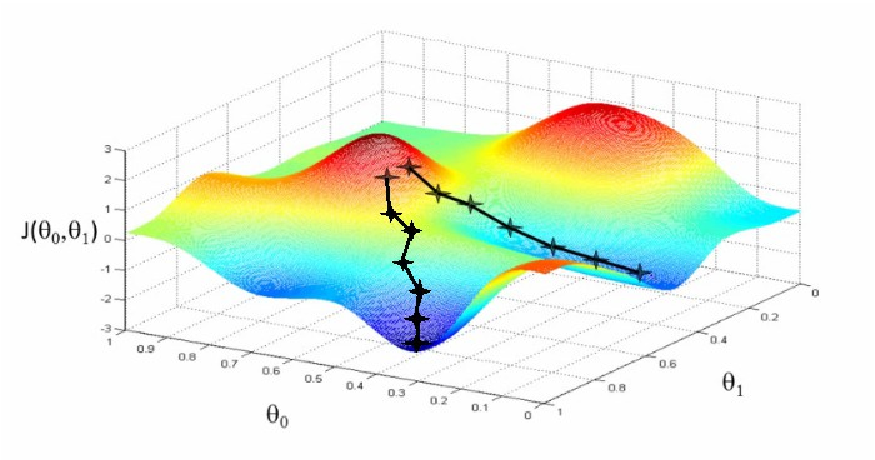
\includegraphics[width=3.5in]{gradient_descent}
\caption{Gradienten Abstiegsverfahren nach Andrew Ng \cite{andrew_ng_17}.}
\label{fig:gradient_descent}
\end{figure}

\subsection{Zielfunktionen}
Die Qualität (Performance) einer Policy berechnet die Zielfunktion (eng. objective function oder criterion) $\rho(\pi)$. R. S. Sutton \cite{sutton_99} unterscheidet zwei verschiedene Formulierungen der Zielfunktion $\rho(\pi)$: 

\begin{equation*}
\begin{aligned}
\rho_{avR}(\pi) & = \lim\limits_{n \rightarrow \infty}{\frac{1}{n} \mathbb{E}\{r_1 + r_2 + ... + r_n | \pi\}} \\
& = \sum_s d^\pi (s) \sum_a \pi(s,a) R^a_s,
\end{aligned}
\end{equation*}

ist die durchschnittliche Belohnung, diese bewertet die Strategie bezüglich der zu erwartenden Langzeitbelohnung pro Schritt. Eine Langzeitbelohnung (eng. long-term reward) ist die Aufsummierung der Belohnungen für eine Entscheidungssequenz. Der Term $d^\pi(s) = \lim\limits_{t \rightarrow \infty} Pr\{s_t = s|s_0,\pi\}$ beschreibt die stationäre Verteilung der Zustände unter $\pi$, d.h. $d^\pi(s)$ gibt an, wie hoch die Wahrscheinlichkeit dafür ist, jeden Zustand $s_t$ zu erreichen, bedingt durch die Policy $\pi$ und unabhängig vom Startzustand $s_0$, wenn $t$ gegen unendlich strebt. Sprachliche Formulierung der Funktion $\rho_{avR}(\pi)$: Es existiert eine Wahrscheinlichkeit, dass sich der Agent in Zustand $s$ befindet und es existiert eine Wahrscheinlichkeit, dass der Agent eine Aktion $a$ auswählt ($a$ abhängig von $\pi$). Berechnet wird die durchschnittliche Belohnung pro Zeitschritt, wobei die Belohnung $R^a_s$ von den beiden vorher erwähnten Wahrscheinlichkeiten $s$ und $a$ abhängt. Der Wert eines Zustands-Aktionspaares, unter Berücksichtigung einer Policy $\pi$, ist für die Zielfunktion der durchschnittlichen Belohnung $\rho_{avR}(\pi)$ wie folgt definiert:

\begin{equation*}
Q^\pi(s,a) = \sum^\infty_{t=1} \mathbb{E}\{r_t - \rho_{avR}(\pi)|s_0 = s, a_0 = a, \pi\},
\end{equation*}

mit $\forall s \in S, a \in A$. Die Funktion berechnet die Summe der Differenzen zwischen einer sofortigen Belohnung ($r_t$) in jedem Zeitschritt $t$ und der Zielfunktion $\rho_{avR}(\pi)$, also der durchschnittlichen Belohnung pro Zeitschritt, für ein Zustands-Aktionspaar unter Verwendung einer Policy $\pi$. R. S. Sutton notiert die Zielfunktion $\rho_{avR}(\pi)$ als $\rho(\pi)$, in dieser Arbeit wird für die durchschnittliche erwartete Belohnung pro Zeitschritt die Notation $\rho_{avR}(\pi)$ verwendet (für \textbf{av}erage \textbf{R}eward ähnlich D. Silver \cite{silver_15}). Die zweite Formulierung der Zielfunktion $\rho(\pi)$ berücksichtigt einen genau festgelegten Startzustand $s_0$ und ausschließlich von diesem Startzustand ausgehende Langzeitbelohnungen:

\begin{equation*}
\rho_{s_0}(\pi) = \mathbb{E}\{\sum^\infty_{t=1} \gamma^{t-1} r_t | s_0,\pi \}
\end{equation*}
und
\begin{equation*}
Q^\pi (s,a) = \mathbb{E} \{\sum^\infty_{k=1} \gamma^{k-1} r_{t+k} | s_t = s, a_t = a, \pi\}.
\end{equation*}

Dabei ist $\gamma \in [0,1]$ ein Abschwächungsfaktor ($\gamma = 1$ ist nur in endlichen abzählbaren Sequenzen einzusetzen). Die stationäre Verteilung der Zustände $d^\pi (s)$ ist bei der Startzustandsformulierung eine abgeschwächte Gewichtung der vorgefundenen Zustände angefangen in Zustand $s_0$ und unter Berücksichtigung der Policy $\pi$: $d^\pi (s) = \sum^\infty_{t=0} \gamma^t Pr \{s_t = s | s_0, \pi\}$.
 
\subsection{Bedeutung des Policy Gradient}
Sei $\rho(\theta)$ eine beliebige Strategiezielfunktion. Policy Gradient Algorithmen suchen ein lokales Maximum der Strategiefunktion $\rho(\theta)$, mittels des ansteigenden Gradienten der Strategie, bezüglich der Parameter $\theta$:   
\begin{equation*}
\Delta \theta \approx \alpha \frac{\partial \rho}{\partial \theta} \approx \alpha \nabla_\theta \rho(\theta).
\end{equation*}

Der Gradient der Strategiezielfunktion $\rho(\theta)$ ist der Vektor der partiellen Ableitungen:

\begin{equation*}
\nabla_\theta \rho(\theta) = \frac{\partial \rho}{\partial \theta} =
\begin{pmatrix}
\frac{\partial \rho(\theta)}{\partial \theta_1} \\ 
\vdots \\
\frac{\partial \rho(\theta)}{\partial \theta_n}
\end{pmatrix}.
\end{equation*}

\subsection{Monte-Carlo Policy Gradient}
Das Monte-Carlo Policy Gradient Verfahren berechnet den Gradienten der Strategiefunktion analytisch ohne eine Wertefunktion zu verwenden.

\paragraph*{Softmax Policy} ist eine alternative Darstellung der Strategiefunktion $\pi_\theta(s,a)$ im Gegensatz zu $\epsilon$-geedy. Der Ausdruck $\phi(s,a) \top \theta$ steht für eine Gewichtung von Aktionen, welche lineare Kombination von Merkmalen verwenden. Dieser Ausdruck ergibt einen Wert und der Wert gibt an, wie sehr die konkrete Aktion $a$ bevorzugt ausgewählt werden soll.  $\phi(s,a)$ ist das ausgewählte Merkmal einer Aktion in einem Zustand und $\theta$ ist die Gewichtung dieses Merkmals. Softmax Policy wird ausschließlich für diskrete Aktionsräume verwendet und nicht bei kontinuierlichen Aktionsräumen. Um den Ausdruck $\phi(s,a) \top \theta$ in eine Wahrscheinlichkeit umzuwandeln, wird dieser exponenziert und normalisiert.

\begin{equation*}
\pi_\theta(s,a) \propto e^{\phi(s,a) \top \theta}
\end{equation*}

d.h. die Wahrscheinlichkeit das die Aktion $a$ wirklich ausgewählt wird, ist Proportional zum exponenzierten Wert der gewichteten linearen Kombination der Merkmale. Eine lineare Kombination von Merkmalen in z.B. einem Labyrinth mit einem diskreten Aktionsraum von Hoch, Runter, Links und Rechts: Jede der Vier Aktionen erhält Merkmale, je höher die Punktzahl (eng. score) der Merkmale ist, wenn die gewichtete Summe der linearen Merkmale berechnet wird, desto höher ist die Wahrscheinlichkeit die Aktion des Merkmals zu wählen.

\paragraph*{Gradient der Softmax Policy (Softmax Score Funktion)} ist die Differenz des Merkmals der tatsächlich ausgewählten Aktion und dem durchschnittlichen Merkmal für alle Aktionen die hätten ausgewählt werden können: 

\begin{equation*}
\nabla_\theta \log \pi_\theta (s,a) = \phi(s,a) - \mathbb{E}_{\pi_\theta}[\phi(s, \cdot)]
\end{equation*}

d.h. die Parameter der Strategiefunktion werden in die Richtung des Gradienten angepasst, wenn das Merkmal der tatsächlich ausgewählten Aktion, im Gegensatz zu allen anderen Merkmalen und deren Aktionen, öfter auftritt (hohe Punktzahl des Merkmals) und eine gute Belohnung erhält. Allgemein ist der Gradient von $\pi_\theta (s,a)$ gleich $\pi_\theta (s,a) \nabla_\theta \log \pi_\theta (s,a)$ nach der Berechnung:

\begin{equation*}
\begin{aligned}
\nabla_\theta \pi_\theta (s,a) & = \pi_\theta (s,a) \frac{\nabla_\theta \pi_\theta (s,a)}{\pi_\theta (s,a)} \\
& = \pi_\theta (s,a) \nabla_\theta \log \pi_\theta (s,a).
\end{aligned}
\end{equation*}

\paragraph*{Einschritt MDP} ist keine Entscheidungssequenz, sondern ein einziger Zeitschritt in einem MDP. Starte in einem Zustand $s \sim d(s)$, wähle eine Aktion $a$ entsprechend der Strategiefunktion $\pi_\theta(s,a)$ und erhalte eine Belohnung definiert durch die Funktion $R^a_s$:

\begin{equation*}
J(\theta) = \mathbb{E}[R_{s,a}] = \sum_{s \in S} d(s) \sum_{a \in A} \pi_\theta(s,a) R_{s,a}.
\end{equation*}

Die Schreibweise $J(\theta)$ der Zielfunktion $\rho_{avR}(\theta)$ ist von D. Silver \cite{silver_15}, daher $J(\theta) \sim \rho_{avR}(\pi)$. Der Gradient dieser Zielfunktion ist entsprechend:

\begin{equation*}
\begin{aligned}
\nabla_\theta J(\theta) & = \sum_{s \in S} d(s) \sum_{a \in A} \pi_\theta(s,a) \nabla_\theta \log \pi_\theta(s,a) R_{s,a} \\
& = \mathbb{E}_{\pi_\theta}[\nabla_\theta \log \pi_\theta(s,a) R_{s,a}],
\end{aligned}
\end{equation*}

d.h. einzig die Policy $\pi_\theta(s,a)$ ist abhängig von $\theta$, darum muss der Gradient nur von dieser Policy gebildet werden. Dieser Aktualisierungsschritt benötigt kein Modell, denn die Policy $\pi_\theta(s,a)$ ist bekannt. $\mathbb{E}_{\pi_\theta}[\nabla_\theta \log \pi_\theta(s,a) R_{s,a}]$ bedeutet: Der Erwartungswert $\mathbb{E}$ unterliegt einer Strategiefunktion $\pi_\theta$, sprich er ist abhängig von einem Startzustand $s$ und einer ausgewählten Aktion $a$ der Strategiefunktion $\pi_\theta(s,a)$. Der durch die Strategiefunktion bedingte Erwartungswert wird berechnet durch den Erwartungswert von $\nabla_\theta \log \pi_\theta(s,a)$ (Punktzahl) multipliziert mit der sofortigen Belohnung (eng. immediate reward) $R_{s,a}$. 

\paragraph*{Policy Gradient Theorem} ist die Substitution der sofortigen Belohnung $R_{s,a}$ mit der Langzeitbelohnung $Q^{\pi_\theta}(s,a)$ aus der Berechnung des Gradienten der Zielfunktion:

\begin{equation*}
\nabla_\theta J(\theta) = \mathbb{E}_{\pi_\theta}[\nabla_\theta \log \pi_\theta(s,a) Q^{\pi_\theta}(s,a)],
\end{equation*}

Das Policy Gradient Theorem verallgemeinert das Einschritt MDP auf eine Sequenz von Zeitschritten (Mehrfachschritt MDP). Das Theorem ist auf die Startzustandszielfunktion und auf die durchschnittliche Langzeitbelohnung Zielfunktion anwendbar. Ein Nachteil dieses Verfahrens ist die relativ hohe Varianz. Das Actor-Critic Policy Gradient Verfahren (detaillierte Informationen von u.a. R. S. Sutton \cite{sutton_barto_12} und D. Silver \cite{silver_15}) verwendet eine Strategiefunktionen und eine Wertefunktionen für das lernen/aktualisieren der Parametervektoren und verringert somit die Varianz. Das Actor-Critic Verfahren ist sehr fortgeschritten und wird oft in der Praxis eingesetzt. Auf eine genaue Erläuterung dieses Verfahrens muss auf Grund des begrenzten Umfangs dieser Arbeit verzichtet werden.


% use section* for acknowledgment
%\section*{Acknowledgment}


%The authors would like to thank...





% trigger a \newpage just before the given reference
% number - used to balance the columns on the last page
% adjust value as needed - may need to be readjusted if
% the document is modified later
%\IEEEtriggeratref{8}
% The "triggered" command can be changed if desired:
%\IEEEtriggercmd{\enlargethispage{-5in}}

% references section

% can use a bibliography generated by BibTeX as a .bbl file
% BibTeX documentation can be easily obtained at:
% http://mirror.ctan.org/biblio/bibtex/contrib/doc/
% The IEEEtran BibTeX style support page is at:
% http://www.michaelshell.org/tex/ieeetran/bibtex/
%\bibliographystyle{IEEEtran}
% argument is your BibTeX string definitions and bibliography database(s)
%\bibliography{IEEEabrv,../bib/paper}
%
% <OR> manually copy in the resultant .bbl file
% set second argument of \begin to the number of references
% (used to reserve space for the reference number labels box)

\begin{thebibliography}{1}

\bibitem{sutton_barto_12}
R.~S. Sutton and A.~G. Barto,
\emph{Reinforcement Learning: An Introduction}, 2rd~ed.\hskip 1em plus
  0.5em minus 0.4em\relax Cambridge, Massachusetts, London, England: MIT Press, 2012.
 
\bibitem{sutton_99}
R.~S. Sutton and D.~ McAllester and S.~Singh and Y.~Mansour,
\emph{Policy Gradient Methods for Reinforcement Learning with Function Approximation}, 180 Park Avenue, Florham Park, NY 07932: AT\&T Labs, 1999.

\bibitem{hoever_14}
G.~ Hoever, \emph{Höhere Mathematik kompakt}, 2. Auflage, Springer Spektrum, 2014.

\bibitem{silver_15}
D.~ Silver, \emph{Online Course Reinforcement Learning}, http://www0.cs.ucl.ac.uk/staff/d.silver/web/Teaching.html, London, England: Googel Deep Mind, 2015.

\bibitem{andrew_ng_17}
A.~ Ng, \emph{01 and 02: Introduction, Regression Analysis and Gradient Descent}, http://www.holehouse.org/mlclass, Stanford University Lectures, 2017.

\bibitem{goodfellow_16}
I.~Goodfellow and Y.~Bengio and A.~Courville,
\emph{Deep Learning}, MIT Press, 2016.


\end{thebibliography}



% that's all folks
\end{document}


